
上一节的结果可能会有些沮丧。处理器非常复杂,需要处理很多问题才能以最高效率运行。这里,我们从简单的开始,看看处理器基本操作的速度。为此,我们将使用谷歌基准测试工具。下面是两个数组简单相加的基准测试:

\hspace*{\fill} \\ %插入空行
\noindent
\textbf{01\_superscalar.C}
\begin{lstlisting}[style=styleCXX]
#include "benchmark/benchmark.h"
void BM_add(benchmark::State& state) {
	srand(1);
	const unsigned int N = state.range(0);
	std::vector<unsigned long> v1(N), v2(N);
	for (size_t i = 0; i < N; ++i) {
		v1[i] = rand();
		v2[i] = rand();
	}
	unsigned long* p1 = v1.data();
	unsigned long* p2 = v2.data();
	for (auto _ : state) {
		unsigned long a1 = 0;
		for (size_t i = 0; i < N; ++i) {
			a1 += p1[i] + p2[i];
		}
		benchmark::DoNotOptimize(a1);
		benchmark::ClobberMemory();
	}
	state.SetItemsProcessed(N*state.iterations());
}
BENCHMARK(BM_add)->Arg(1<<22);
BENCHMARK_MAIN();
\end{lstlisting}

第一个例子,展示了基准的所有细节,包括输入的生成。大多数操作的速度并不依赖于操作数的值,这里使用随机输入,这样在处理对输入敏感的操作时就不用担心了。虽然将值存储在数组中,但我们不想测试数组索引的速度:编译器肯定会优化表达式\texttt{v1[i]},以生成与\texttt{p1[i]}完全相同的代码,但为什么要冒这个险呢?将尽可能多的不重要的细节排除在外,直到剩下最基本的问题。内存中有两个数组,我们想对数组的每个元素进行一些计算。

另一方面,必须考虑不需要的编译器优化的可能。编译器可能会发现整个程序只是一个非常长,且什么都不做的过程(至少就C++标准而言是这样的),并通过优化掉大块的代码,给出一个更快的方法来做同样的事情。编译器的方向是不要优化掉计算的结果,并假定内存的状态可以在基准迭代之间进行修改,这也会阻止此类优化。另外,将变量\texttt{a1}声明为\texttt{volatile}肯定会阻止大多数不应该的优化。反过来,它也会阻止编译器优化循环,这不是我们想要的结果。我们想看到CPU如何高效地处理两个数组,也就是如何生成最高效的代码。我们只是不想让编译器发现基准循环的第一次迭代与第二次迭代完全相同。

微基准测试的一个不寻常的应用。有一小段代码,我们想知道它有多快,以及如何使它更快。我们使用微基准来了解处理器的性能,通过对代码进行裁剪,带给一些启发。

编译基准测试时,应该打开优化选项。运行基准测试将产生如下的结果(当然确切的数字取决于CPU):

%\hspace*{\fill} \\ %插入空行
\begin{center}
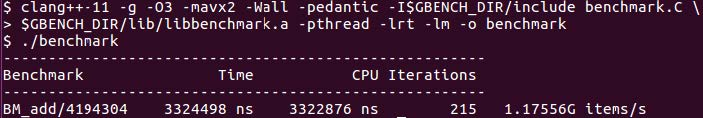
\includegraphics[width=0.9\textwidth]{content/1/chapter3/images/2.jpg}\\
图 3.2
\end{center}

目前,我们还不能从这个实验中得出什么结论(除了现代CPU速度的确快)。CPU可以在不到1纳秒的时间内将两个数字相加。如果对此感到好奇,可以探索一下其他运算:减法和乘法所花费的时间与加法相同,而整数除法则相当缓慢(比加法慢三到四倍)。

为了分析代码的性能,必须按照处理器的方式来进行。两个输入数组存储在内存中,但是加法或乘法操作是在存储在寄存器中的值之间执行的(对于某些操作,可能是在寄存器和内存位置之间)。这就是处理器如何一步步地对循环进行迭代。迭代开始时,索引变量\texttt{i}在一个CPU寄存器中,对应的两个数组元素\texttt{v1[i]}和\texttt{v2[i]}在内存中:

%\hspace*{\fill} \\ %插入空行
\begin{center}
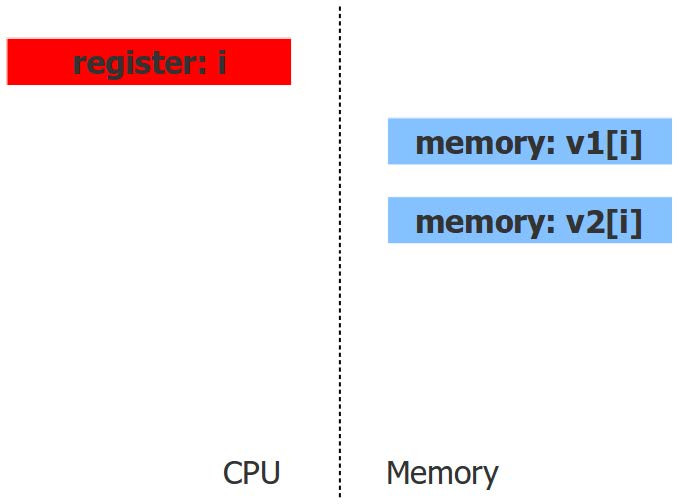
\includegraphics[width=0.6\textwidth]{content/1/chapter3/images/3.jpg}\\
图 3.3
\end{center}

做计算之前,必须将输入移到寄存器中。必须为每个输入分配一个寄存器,并为结果分配一个寄存器。在给定的循环迭代中,第一个指令会把一个输入加载到寄存器中:

%\hspace*{\fill} \\ %插入空行
\begin{center}
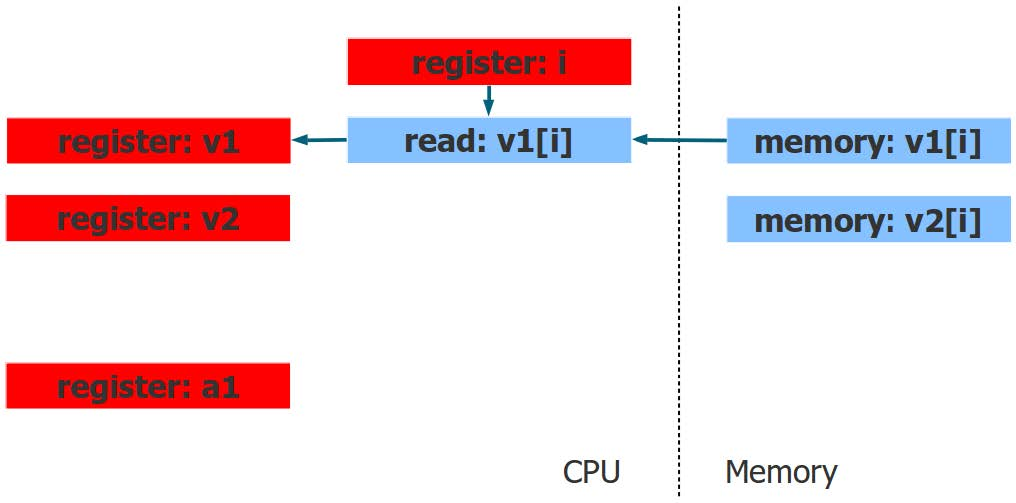
\includegraphics[width=0.7\textwidth]{content/1/chapter3/images/4.jpg}\\
图3.4 - 第i次迭代:第一个指令后的处理器状态
\end{center}

read(或load)指令使用内存中包含索引\texttt{i}和数组\texttt{v1}位置的寄存器来访问值\texttt{v1[i]},并将其复制到寄存器中。下一条指令以相同的方式来加载第二个输入:

%\hspace*{\fill} \\ %插入空行
\begin{center}
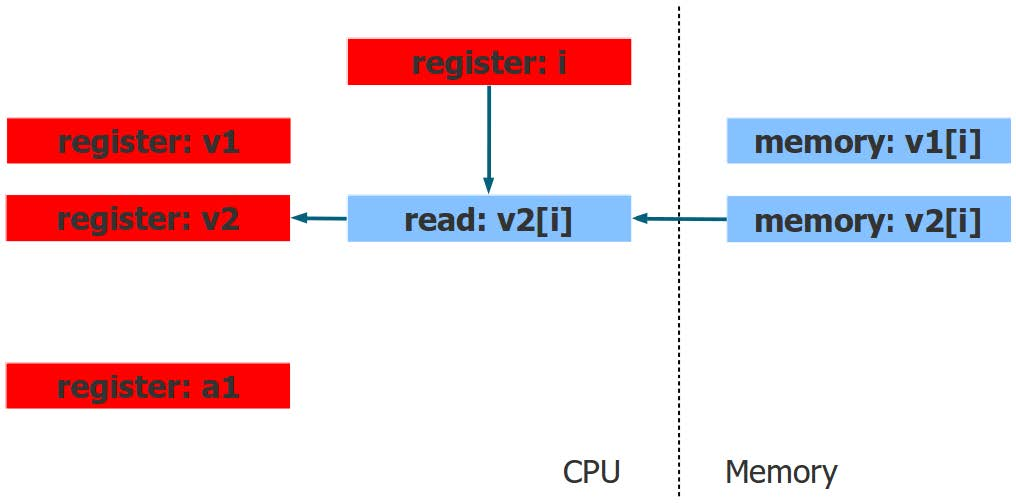
\includegraphics[width=0.7\textwidth]{content/1/chapter3/images/5.jpg}\\
图3.5 - 第i次迭代:第2条指令后的处理器状态
\end{center}

现在可以进行加法或乘法运算了:

%\hspace*{\fill} \\ %插入空行
\begin{center}
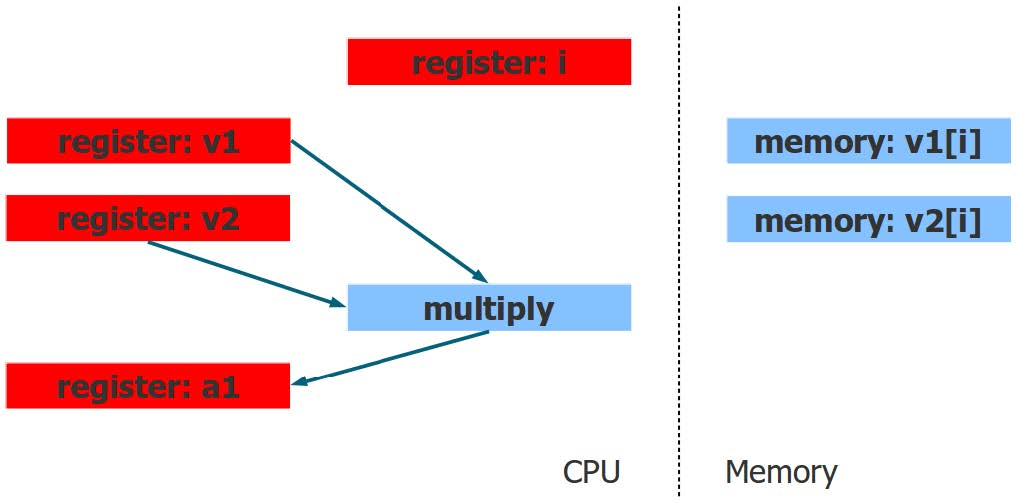
\includegraphics[width=0.7\textwidth]{content/1/chapter3/images/6.jpg}\\
图3.6 -第i次循环迭代结束时的处理器状态
\end{center}

这行简单的代码在转换成硬件指令后,就产生了所有这些操作(加上进入下一次循环迭代所需的操作):

\begin{lstlisting}[style=styleCXX]
a1 += p1[i] + p2[i];
\end{lstlisting}

从效率的角度来看,我们只关注最后一步。CPU可以在一纳秒内把两个数字相加或相乘,这已经很好了,但还能做得更好吗?许多晶体管都致力于处理和执行指令,所以它们能处理更多的东西。让我们尝试对相同的值做两个操作,而不是一个:

\hspace*{\fill} \\ %插入空行
\noindent
\textbf{01\_superscalar.C}
\begin{lstlisting}[style=styleCXX]
void BM_add_multiply(benchmark::State& state) {
	… prepare data …
	for (auto _ : state) {
		unsigned long a1 = 0, a2 = 0;
		for (size_t i = 0; i < N; ++i) {
			a1 += p1[i] + p2[i];
			a2 += p1[i] * p2[i];
		}
		benchmark::DoNotOptimize(a1);
		benchmark::DoNotOptimize(a2);
		benchmark::ClobberMemory();
	}
	state.SetItemsProcessed(N*state.iterations());
}
\end{lstlisting}

如果加法和乘法都需要1纳秒,那么两者都需要多长时间?基准测试给了我们答案:

%\hspace*{\fill} \\ %插入空行
\begin{center}
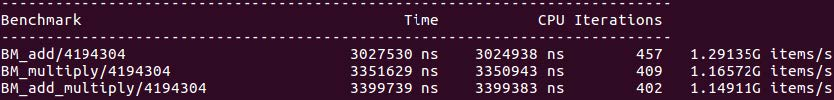
\includegraphics[width=0.9\textwidth]{content/1/chapter3/images/7.jpg}\\
图3.7 - 一条指令和两条指令的基准测试
\end{center}

令人惊讶的是,这里一加一,居然等于一。我们可以在一次迭代中添加更多的指令:

\begin{lstlisting}[style=styleCXX]
for (size_t i = 0; i < N; ++i) {
	a1 += p1[i] + p2[i];
	a2 += p1[i] * p2[i];
	a3 += p1[i] << 2;
	a4 += p2[i] – p1[i];
}
\end{lstlisting}

每次迭代的时间仍然相同(基准测量的精度范围内略有差异):

%\hspace*{\fill} \\ %插入空行
\begin{center}
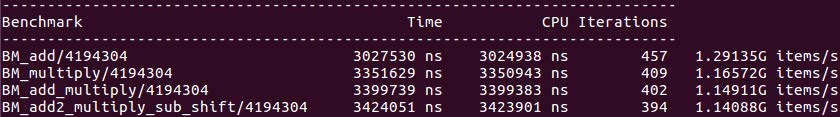
\includegraphics[width=0.9\textwidth]{content/1/chapter3/images/8.jpg}\\
图3.8 - 每次迭代最多有四条指令循环的基准测试结果
\end{center}

我们认为处理器每次只执行一条指令的观点需要修正了:

\hspace*{\fill} \\ %插入空行
\begin{center}
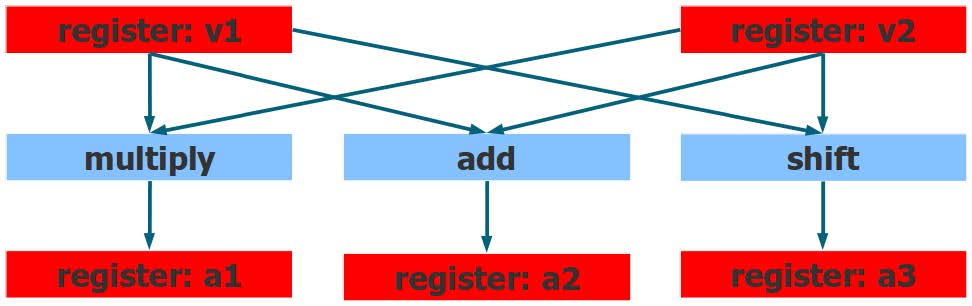
\includegraphics[width=0.9\textwidth]{content/1/chapter3/images/9.jpg}\\
图3.9 - 处理器在一次执行多个操作
\end{center}

只要操作数在寄存器中了,处理器就可以同时执行多个操作,这就是所谓的\textbf{指令级并行(ILP)}。当然,可以执行多少操作是有限制的,处理器能够执行整数的计算单元是有限的。尽管如此,通过在一次迭代中添加越来越多的指令,尝试将CPU推向极限是有指导意义的:

\begin{lstlisting}[style=styleCXX]
for (size_t i = 0; i < N; ++i) {
	a1 += p1[i] + p2[i];
	a2 += p1[i] * p2[i];
	a3 += p1[i] << 2;
	a4 += p2[i] – p1[i];
	a5 += (p2[i] << 1)*p2[i];
	a6 += (p2[i] - 3)*p1[i];
}
\end{lstlisting}

当然,处理器可以执行的指令数量取决于CPU和指令,但与单个乘法运算相比,前面的循环速度明显出现了下降,至少在我使用的机器上是这样:

%\hspace*{\fill} \\ %插入空行
\begin{center}
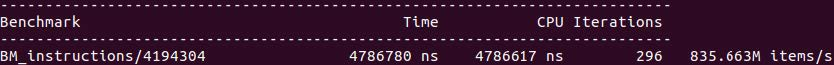
\includegraphics[width=0.9\textwidth]{content/1/chapter3/images/10.jpg}\\
图3.10 - 每迭代8条指令的基准测试结果
\end{center}

就硬件利用率而言,可以看到最初的代码是多么低效。CPU显然可以在每次迭代中执行5到7个不同的操作,因此单个乘法甚至用不到其能力的四分之一。事实上,现代处理器的能力更令人吃惊。除了我们一直在试验的整数计算单元外,还有单独的浮点硬件,可以在双精度或浮点值上执行指令,以及同时执行MMX、SSE、AVX和其他专门指令的向量处理单元!

\subsubsubsection{3.3.1\hspace{0.2cm}可视化的指令级并行}

目前,我们关于CPU并行执行多条指令能力的结论还是基于间接证据。如果能直接确认这就是事实,那就太好了。我们可以从\textbf{机器码分析器(MCA)}得到这样的确认,它是LLVM工具链的一部分。分析器将汇编代码作为输入,并获得关于指令如何执行、延迟和瓶颈是什么等信息。我们不打算在这里学习这个高级工具的功能(详细信息请参阅项目主页,\url{https://llvm.org/docs/CommandGuide/llvm-mca.html})。现在,可以使用它来查看CPU如何执行操作的。

第一步是用分析器标记注释代码,选择要分析的代码段:

\begin{lstlisting}[style=styleCXX]
#define MCA_START __asm volatile("# LLVM-MCA-BEGIN");
#define MCA_END __asm volatile("# LLVM-MCA-END");
…
for (size_t i = 0; i < N; ++i) {
MCA_START
	a1 += p1[i] + p2[i];
MCA_END
}
\end{lstlisting}

不必为分析器标记使用\texttt{\#define},但记住这些命令比记住精确的汇编语法要容易(可以保存\texttt{\#define}在头文件中,并在需要时包含)。为什么只标记循环的主体,而不是整个循环呢?分析器实际上假设所选的代码片段在一个循环中运行,并将其重复若干次迭代(默认情况下为10次)。可以尝试为分析标记整个循环。但根据编译器的优化,这可能会使分析器感到困惑(这是一个强大的工具,但不容易使用)。

现在运行分析器:

%\hspace*{\fill} \\ %插入空行
\begin{center}
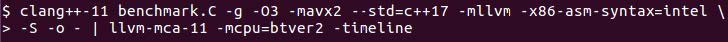
\includegraphics[width=0.9\textwidth]{content/1/chapter3/images/11.jpg}\\
图 3.11
\end{center}

我们不是把代码编译成可执行文件,而是用Intel语法生成汇编输出(\texttt{-S})。输出输送到分析器,在分析器可以报告结果的许多方式中,我们选择了时间轴输出。时间轴视图显示每条指令在执行过程中的移动。我们分析两个代码片段,一个使用单个操作(加法或乘法),另一个使用两个操作。以下是迭代的时间线,只有一次乘法(我们已经删除了时间线中间的所有行):

%\hspace*{\fill} \\ %插入空行
\begin{center}
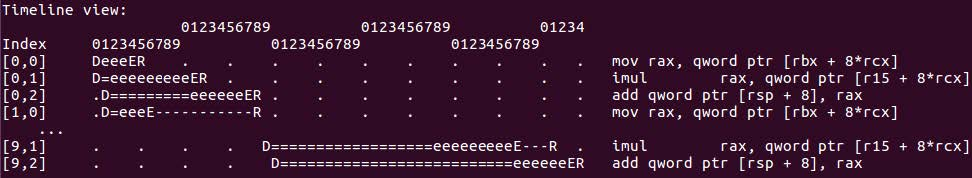
\includegraphics[width=0.9\textwidth]{content/1/chapter3/images/12.jpg}\\
图 3.12
\end{center}

横轴是时的周期,该分析模拟运行选定的代码片段十次迭代,每条指令都由其在代码中的序号和迭代索引来标识,因此第一次迭代的第一条指令的索引为[0,0],最后一条指令的索引为[9,2]。最后一条指令也是第十次迭代的第三条指令(每次迭代只有三条指令)。根据时间轴,整个过程需要55个周期。

从内存中读取\texttt{p1[i]}和\texttt{p2[i]},对其进行操作:

\begin{lstlisting}[style=styleCXX]
#define MCA_START __asm volatile("# LLVM-MCA-BEGIN");
#define MCA_END __asm volatile("# LLVM-MCA-END");
…
for (size_t i = 0; i < N; ++i) {
MCA_START
	a1 += p1[i] + p2[i];
	a2 += p1[i] * p2[i];
MCA_END
}
\end{lstlisting}

让我们看看每个迭代有两个操作的时间轴,一个加法和一个乘法:

%\hspace*{\fill} \\ %插入空行
\begin{center}
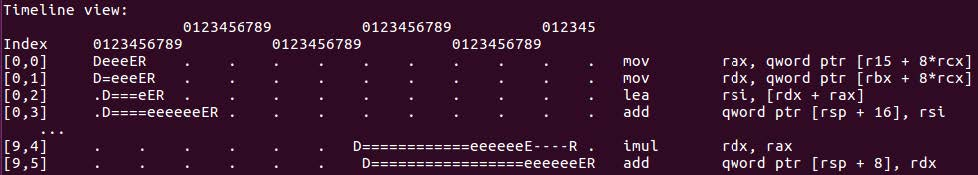
\includegraphics[width=0.9\textwidth]{content/1/chapter3/images/13.jpg}\\
图 3.13
\end{center}

现在执行的指令更多了,每次迭代有6条指令(最后一条指令有索引[9,5])。时间轴的持续时间只增加了一个周期。图3.12中,时间轴结束于第54周期,而在图3.13中,结束于第55周期。正如我们所怀疑的那样,处理器在同样长的时间内执行了两倍的指令。

可能还注意到,对于目前为止的所有基准测试,我们都增加了对相同输入值执行的操作的数量(添加、减去、乘以等)。就运行时而言,这些额外的操作是免费的(在一定程度上),这是非常重要的经验:当在寄存器中有了一些值,在相同的值上加法计算可能不会降低任何性能,除非程序已经非常高效,并且将硬件压到了极限。遗憾的是,实验和结论的实用价值有限。所有计算在同一时间只执行少量输入,下一次迭代使用自己的输入,并且可以在相同的输入上找到一些更有用的计算,这种情况发生的频率有多高呢?也不是没有,但很少。扩展我们对CPU计算能力的简单演示将会遇到一个或多个难题,首先就是数据依赖。循环的顺序迭代通常不独立,可能每个迭代都需要一些来自前面迭代的数据。下一节将探讨这种情况。

















